\section{Future Works}\label{sec:future_Work}
The current work in progress aims at scaling the current resilience planning framework to solve large-scale optimization model in terms of resources, network, and scenario under consideration. As discussed in our existing work, the scenarios are time and space varying and hence such details are necessary to be incorporated in the planning model for better accuracy. Additionally, solving the extensive form of the problem is suffered by the curse of dimensionality. Hence, off-the-shelf solvers are more likely to crash or provide high optimality gap solutions when high dimensionalo extensive form of the model is fed to the solvers. Thus, solving a large-scale stochastic optimization problem has several challenges and is an active area of research that motivates us in our future work. In addition, operational planning strategies like defensive islanding would be studied to better prepare with the upcoming hurricane storms. Such proactive islanding method can prevent the propagation of cascading failure effects in the power system.

\subsection{Large-scale Resilience Planning Framework}
\subsubsection{Multiple-resource Resilience Planning using Scenario-based Dual Decomposition}
Our existing planning model plans for the DG siting and sizing problem for a range of stochastic wind events. However, the infrastructures planning problem can have multiple portfolio of resources including remote-controlled switches (RCS) and line hardening measures. There are existing works using several other planning measures as such~\cite{7514755}. However, as discussed earlier, such methods plan for the expected events but not for HILP events. The objective of this task is to formulate a planning model with multiple resources and observe the trade-off of planning among these multiple resources considering budget constraints. A dual decomposition-based algorithm will be studied to solve the scenario-based sub-problems in parallel by leveraging high-performance computing (HPC) platforms. Although such algorithms are heuristically driven, several convergence  and bounding guarantees exist in the literature for such algorithms~\cite{boland2018combining}.   

\subsubsection{Hub and Spoke Architecture for Scalable and Parallel Implementation of Stochastic Optimization}
Although parallel algorithms are faster in solving the stochastic optimization problem they can run into bottlenecks when individual sub-problems are hard to solve. In such a case, communication overhead can outweigh the parallel speedup. Such problems can rather take more time than serial methods as subproblems that have finished their work need to wait for other subproblems that have not. Hence, the objective of this task is to explore asynchronous parallel algorithm based on hub and spoke architecture as suggested in~\cite{knueven2020parallel}. When solved in hub and spoke architecture, the problems can be independently solved with less or no communication. This asynchronous problem-solving behavior increases the parallel speedup significantly. 

\subsection{Defensive Islanding and Restoration of Electric Power Systems Against Extreme Weather Events}
Extreme weather event, such as hurricane and storm surge, can have devastating impacts on the power grid and can result in cascading failures of the resources if not handled properly. During an upcoming storm, it is typically difficult to address the operational decisions considering the timescale of the events and resources required. However, it is possible to minimize the impact of these events if the grid is splitted into multiple self-sustaining islands ahead of the event. There are some existing works proposing the idea of defensive islanding. However, the event scenarios in these works are non-realistic as the spatiotemporal impact of these events are not considered. The aim of this work is to propose a defensive islanding strategy to minimize the spatiotemporal impact of extreme weather events. Furthermore, restorative actions will also be implemented once the event settles after some time.    

%\begin{comment}
\clearpage
\subsection{Timeline}
The time-line for the research efforts as detailed in Section~\ref{sec:future_Work} is shown in Fig. \ref{fig:time}.

\begin{figure}[h!]
\centering
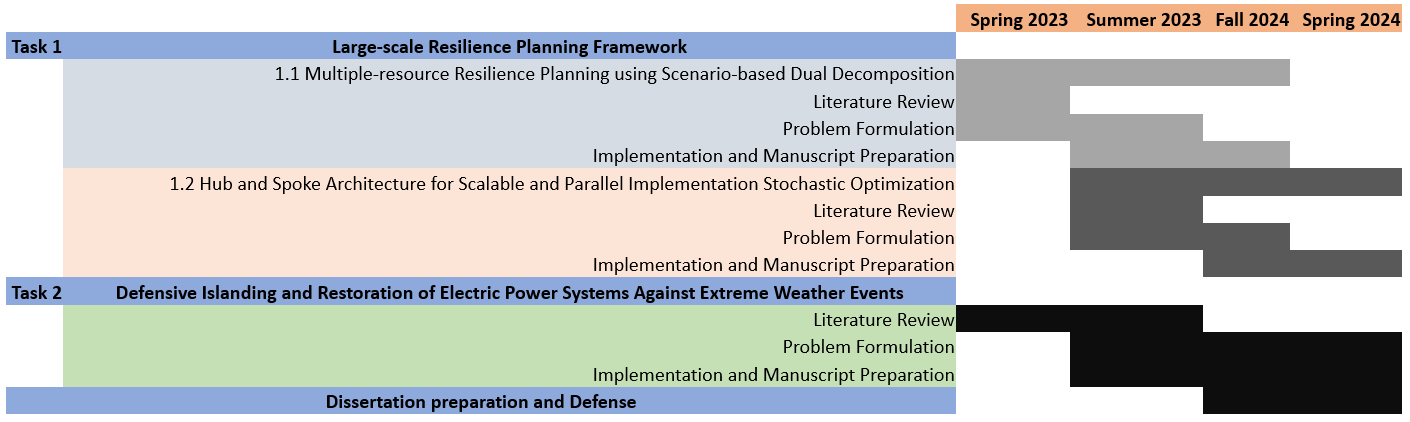
\includegraphics[width=\linewidth]{figures/timeline.PNG}
  \vspace{-0.2 cm}
  \caption{\small Gantt chart showing execution plan for future works.}
\label{fig:time}
\end{figure}
